%\VignetteIndexEntry{GGtools overview}
%\VignetteDepends{}
%\VignetteKeywords{Genetical genomics,SNP,expression}
%\VignettePackage{GGtools}

%
% NOTE -- ONLY EDIT THE .Rnw FILE!!!  The .tex file is
% likely to be overwritten.
%
\documentclass[12pt]{article}

\usepackage{amsmath,pstricks}
\usepackage[authoryear,round]{natbib}
\usepackage{hyperref}


\textwidth=6.2in
\textheight=8.5in
%\parskip=.3cm
\oddsidemargin=.1in
\evensidemargin=.1in
\headheight=-.3in

\newcommand{\scscst}{\scriptscriptstyle}
\newcommand{\scst}{\scriptstyle}


\newcommand{\Rfunction}[1]{{\texttt{#1}}}
\newcommand{\Robject}[1]{{\texttt{#1}}}
\newcommand{\Rpackage}[1]{{\textit{#1}}}
\newcommand{\Rmethod}[1]{{\texttt{#1}}}
\newcommand{\Rfunarg}[1]{{\texttt{#1}}}
\newcommand{\Rclass}[1]{{\textit{#1}}}

\textwidth=6.2in

\bibliographystyle{plainnat} 
 
\usepackage{/Users/stvjc/WOrk/ExternalSoft/R-devel/share/texmf/Sweave}
\begin{document}
%\setkeys{Gin}{width=0.55\textwidth}

\title{Overview of \Rpackage{GGtools} for genetical genomics}
\author{VJ Carey \texttt{<stvjc@channing.harvard.edu>}}
\maketitle

\section{Introduction}

We use the term \textit{genetical genomics} to refer to
data analysis activities that link genotypic information
such as SNP configurations to gene expression phenotype.
The \Rpackage{GGtools} package includes various
demonstration resources and analysis tools for these
activities.
We will attach the library and have a look at a basic
demonstration resource.
\begin{Schunk}
\begin{Sinput}
> library(GGtools)
\end{Sinput}
\begin{Soutput}
Loading required package: Biobase
Loading required package: tools
Loading required package: hgfocus
\end{Soutput}
\begin{Sinput}
> data(c20GGceu)
> class(c20GGceu)
\end{Sinput}
\begin{Soutput}
[1] "ggExprSet"
attr(,"package")
[1] ".GlobalEnv"
\end{Soutput}
\begin{Sinput}
> c20GGceu
\end{Sinput}
\begin{Soutput}
GG Expression Set (exprSet catering for many SNP attributes) with 
	8793 genes
	48 samples
There are  114666  attributes; names include:
rs4814683 rs6076506 rs6139074 rs1418258 rs7274499 
\end{Soutput}
\end{Schunk}
The ggExprSet class is an extension of the
\Rclass{exprSet} class.  It represents expression
data from the hgfocus chip on 48 individuals in the CEU
CEPH group, and SNP data obtained from their HapMap genotyping
results.

The data are organized into an 8793
by 48 matrix of expression values
accessible with the \texttt{exprs} method, and
an 48 by 114666
of rare allele counts:
\begin{Schunk}
\begin{Sinput}
> dim(exprs(c20GGceu))
\end{Sinput}
\begin{Soutput}
[1] 8793   48
\end{Soutput}
\begin{Sinput}
> dim(snps(c20GGceu))
\end{Sinput}
\begin{Soutput}
[1]     48 114666
\end{Soutput}
\begin{Sinput}
> snps(c20GGceu)[1:5, 1:5]
\end{Sinput}
\begin{Soutput}
        rs4814683 rs6076506 rs6139074 rs1418258 rs7274499
NA11829         0         2         0         0         2
NA11830         1         2         1         1         1
NA11831         0         2         0         0         2
NA11832         1         2         1         1         2
NA11839         0         2         0         0         2
\end{Soutput}
\end{Schunk}

We need some genetic metadata about SNPs; these are
culled from SNP genotyping panels released on a 
chromosome-by-chromosome basis for CEPH participants
by HapMap project:
\begin{Schunk}
\begin{Sinput}
> data(chr20meta)
> chr20meta[1:4, ]
\end{Sinput}
\begin{Soutput}
      rsnum chrom   pos strand
1 rs4814683 chr20  9795      +
2 rs6076506 chr20 11231      +
3 rs6139074 chr20 11244      +
4 rs1418258 chr20 11799      +
\end{Soutput}
\end{Schunk}

A basic task is to compute a screen (over the genome, or,
more practically, over a chromosome) of genotypic determination
of expression.  The \Rfunction{detScreen} function help
with this; defaults are supplied for an example related to
results in Cheung and Spielman 2005:

\begin{center}
\begin{Schunk}
\begin{Sinput}
> ds1 = detScreen()
\end{Sinput}
\end{Schunk}
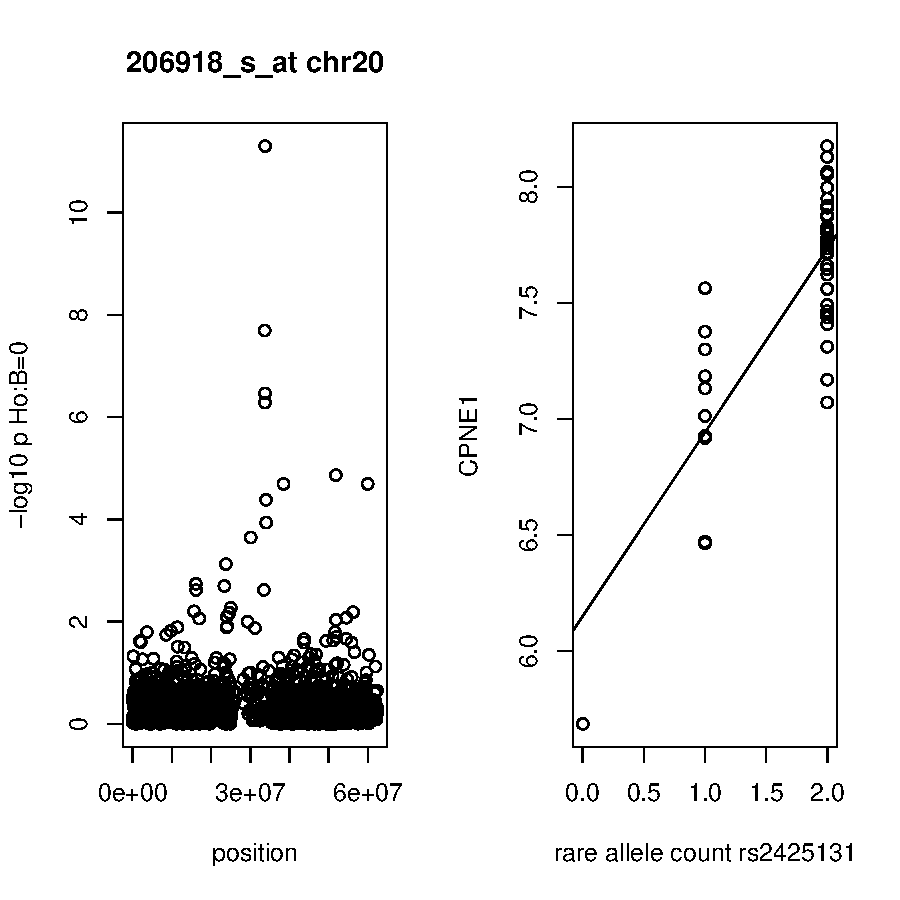
\includegraphics{GGOverview-dosc}
\end{center}

The \Rfunction{detScreen} function returns a list:
\begin{Schunk}
\begin{Sinput}
> names(ds1)
\end{Sinput}
\begin{Soutput}
[1] "bot" "cpn"
\end{Soutput}
\begin{Sinput}
> ds1[[1]]
\end{Sinput}
\begin{Soutput}
rs2425131 
      793 
\end{Soutput}
\begin{Sinput}
> length(ds1[[2]])
\end{Sinput}
\begin{Soutput}
[1] 3
\end{Soutput}
\begin{Sinput}
> names(ds1[[2]])
\end{Sinput}
\begin{Soutput}
[1] "regs"  "pvals" "locs" 
\end{Soutput}
\begin{Sinput}
> ds1[[2]][[1]][[1]]
\end{Sinput}
\begin{Soutput}
Call:
lm(formula = exprs(gge)[psid, ] ~ pData(gge)[[i]])

Coefficients:
    (Intercept)  pData(gge)[[i]]  
        7.51304          0.03847  
\end{Soutput}
\end{Schunk}

\section{Appendix: Package documentation for \Rpackage{GGtools}}
\begin{Schunk}
\begin{Soutput}
		Information on package 'GGtools'

Description:


Package:       GGtools
Title:         software and data for genetical genomics
Version:       0.0-6
Author:        stvjc <stvjc@channing.harvard.edu>
Description:   dealing with hapmap SNP reports, GWAS, etc.
Depends:       R (>= 2.2.0), Biobase, hgfocus
Maintainer:    stvjc <stvjc@channing.harvard.edu>
License:       LGPL
Built:         R 2.4.0; ; 2006-08-07 08:00:25; unix


Index:


c20GGceu                representations of HapMap snp data + expression
                        data
chr20meta               representations of HapMap snp metadata
detScreen               perform a screen for SNP determination of
                        expression using a ggExprSet instance, and
                        produce a plot
geneLocs                gene metadata from NCBI
ggExprSet-class         Class "ggExprSet", representation of genetical
                        genomics (expression + SNP) data
ggreg                   regression analysis for additive effect of
                        genotype on expression
ggrplot                 plot a regression model for additive effect of
                        genotype on expression
regseq                  compute a sequence of regression models
                        relating genotype to expression
snps                    accessor for genotype data in a ggExprSet


Further information is available in the following vignettes in
directory '/Users/stvjc/WOrk/ExternalSoft/R-devel/library/GGtools/doc':


GGoverview: GGtools overview (source)
\end{Soutput}
\end{Schunk}

Session information for this vignette build:
\begin{Schunk}
\begin{Sinput}
> sessionInfo()
\end{Sinput}
\begin{Soutput}
R version 2.4.0 Under development (unstable) (2006-07-16 r38625) 
powerpc-apple-darwin8.7.0 

locale:
C

attached base packages:
[1] "tools"     "methods"   "stats"     "graphics"  "grDevices" "utils"    
[7] "datasets"  "base"     

other attached packages:
  GGtools   hgfocus   Biobase 
  "0.0-6"  "1.12.0" "1.11.20" 
\end{Soutput}
\end{Schunk}

\end{document}
